
\section{Схемы алгоритмов}

\begin{figure}[h!]
	\begin{center}
		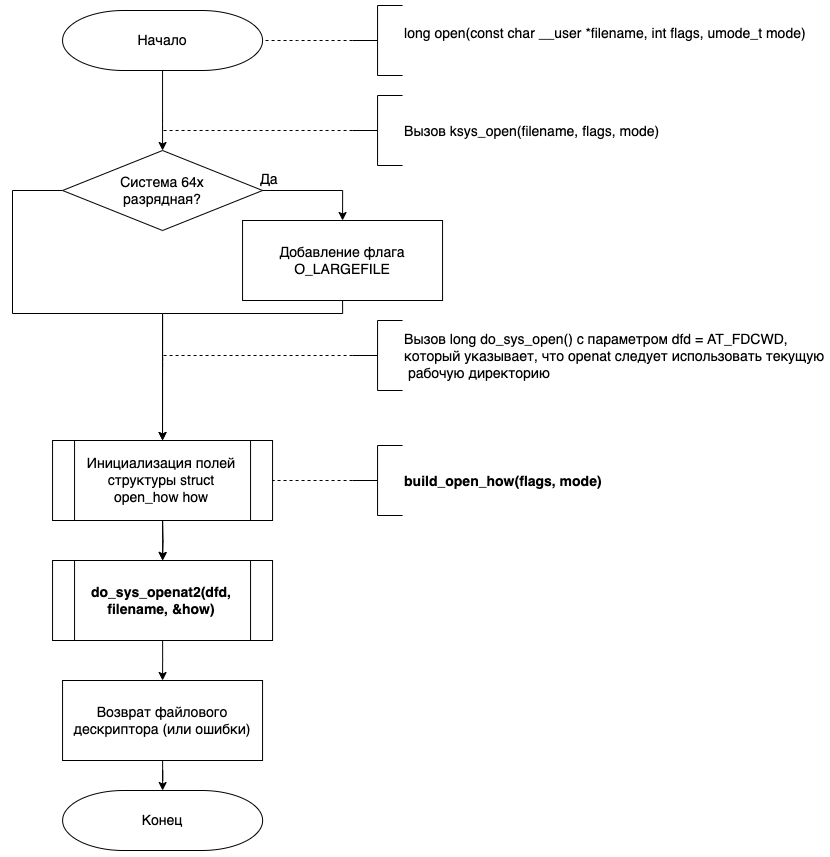
\includegraphics[width=\textwidth]{images/open}
	\end{center}
	\caption{Схема алгоритма работы системного вызова ореn() }
	\label{img:open}
\end{figure}


\begin{figure}[h!]
	\begin{center}
		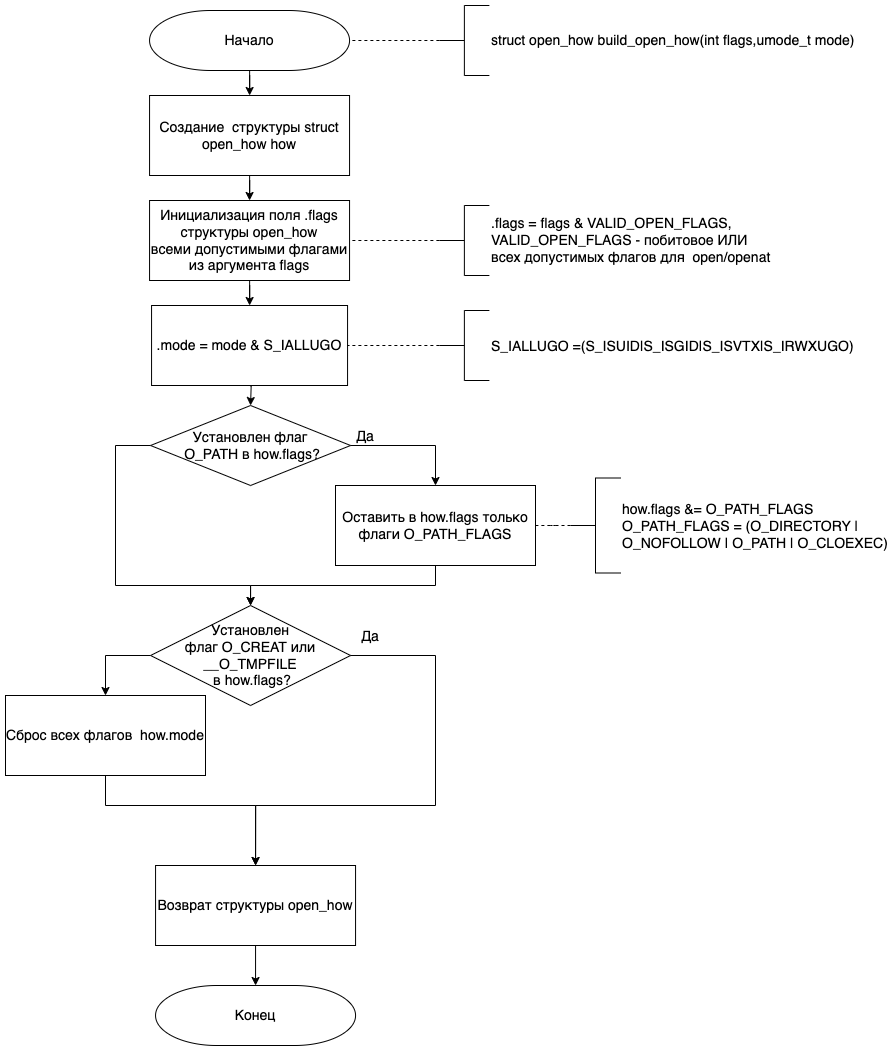
\includegraphics[width=\textwidth]{images/build_open_how}
	\end{center}
	\caption{Схема алгоритма работы функции build\_open\_how() }
	\label{img:open_how}
\end{figure}


\begin{figure}[h!]
	\begin{center}
		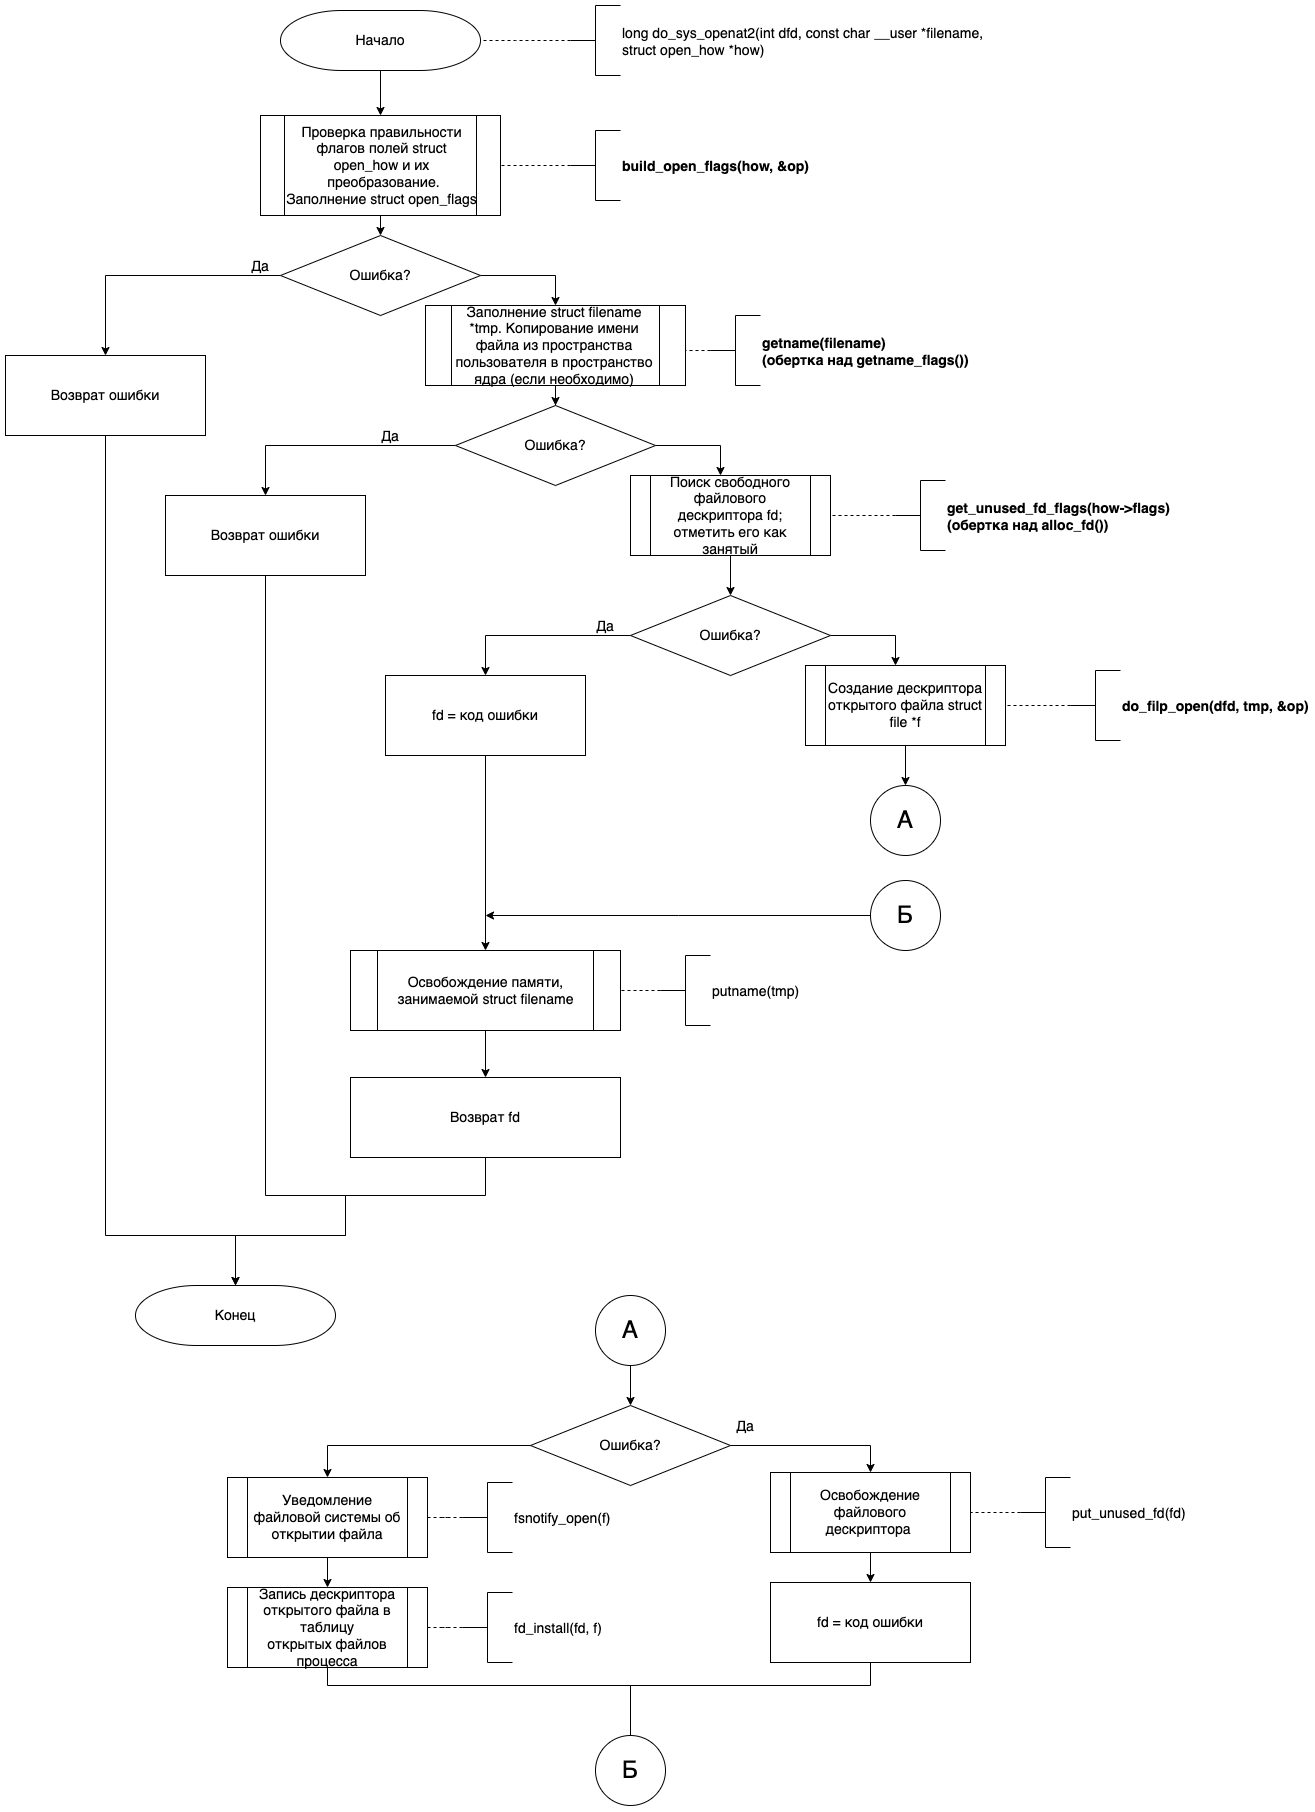
\includegraphics[width=160mm]{images/do_sys_openat2}
	\end{center}
	\caption{Схема алгоритма работы функции do\_sys\_open\_at2() }
	\label{img:openat2}
\end{figure}

\begin{figure}[h!]
	\begin{center}
		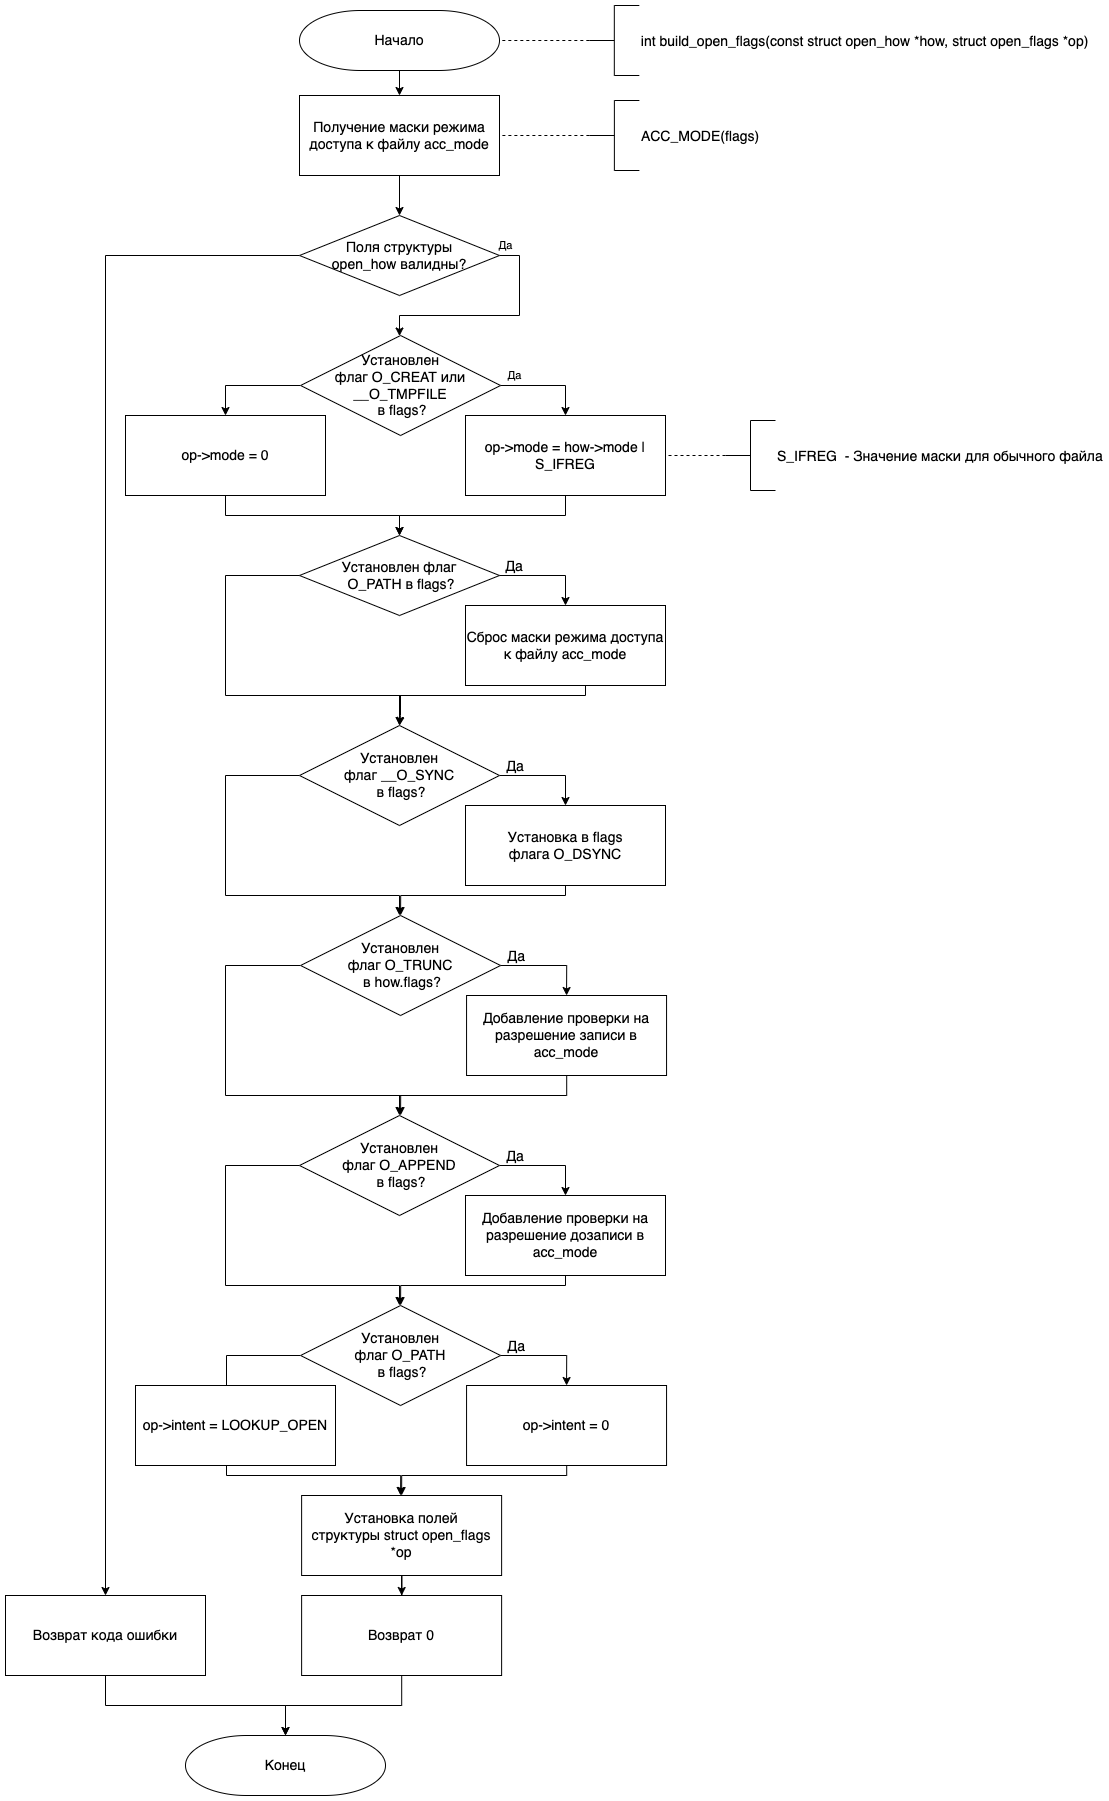
\includegraphics[width=140mm]{images/build_open_flags}
	\end{center}
	\caption{Схема алгоритма работы функции build\_open\_flags() }
	\label{img:build_open}
\end{figure}


\begin{figure}[h!]
	\begin{center}
		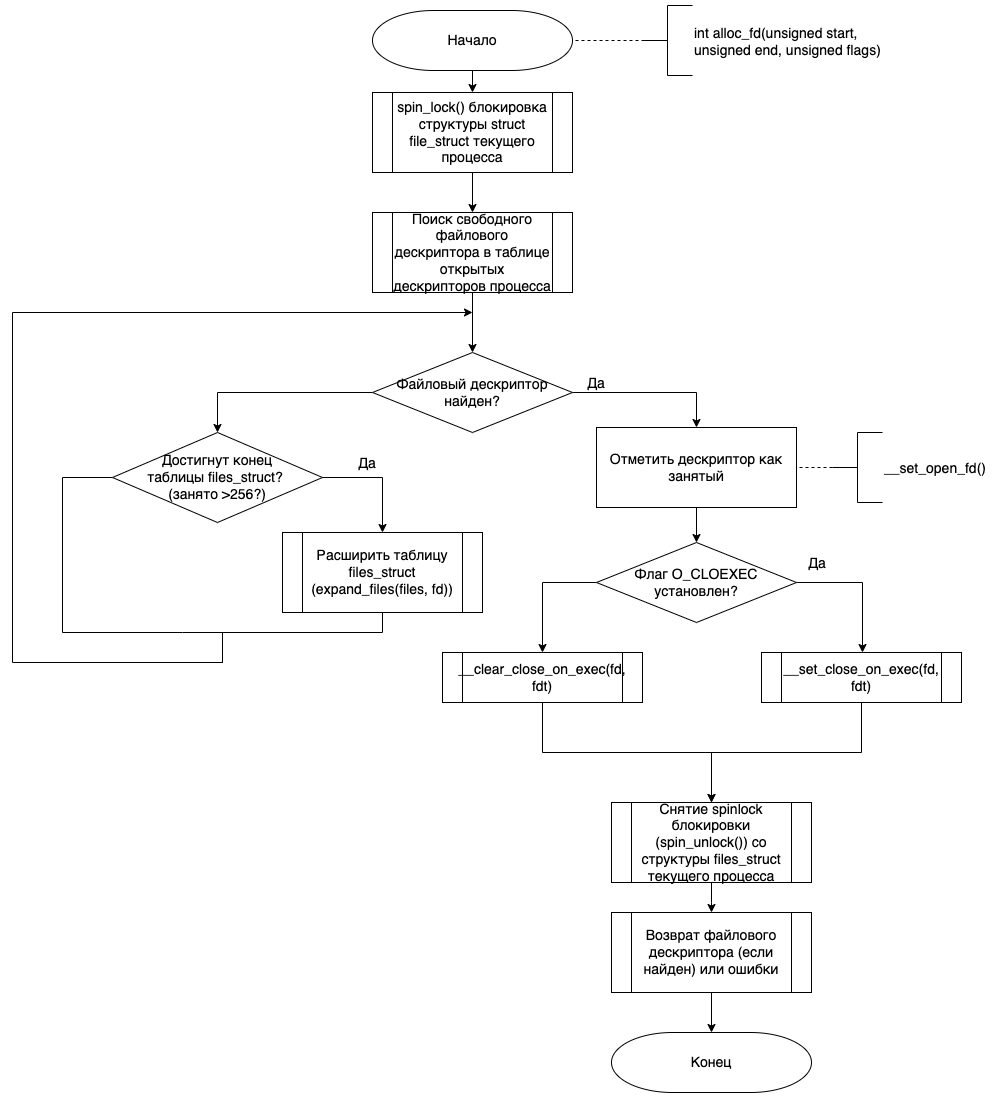
\includegraphics[width=\textwidth]{images/alloc_fd}
	\end{center}
	\caption{Схема алгоритма работы функции alloc\_fd()}
	\label{img:alloc}
\end{figure}

\begin{figure}[h!]
	\begin{center}
		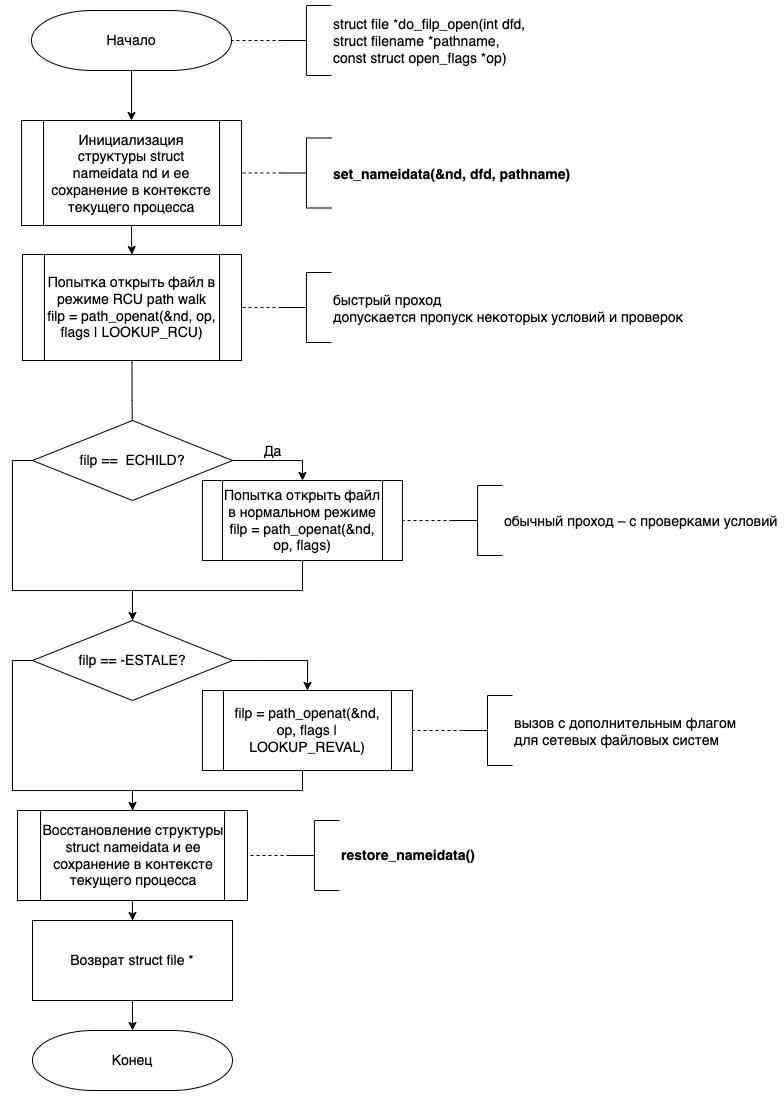
\includegraphics[width=140mm]{images/do_filp_open}
	\end{center}
	\caption{Схема алгоритма работы функции do\_filp\_open()}
	\label{img:flip}
	
	 \textit{LOOKUP\_RCU} -- флаг используется в системе VFS  для указания , что операция поиска должна выполняться с использованием RCU (Read-Copy-Update). 
	
	\textit{LOOKUP\_REVAL} --  флаг для работы с NFS, указывает, что необходимо выполнить повторную проверку.
	
\end{figure}


\begin{figure}[h!]
	\begin{center}
		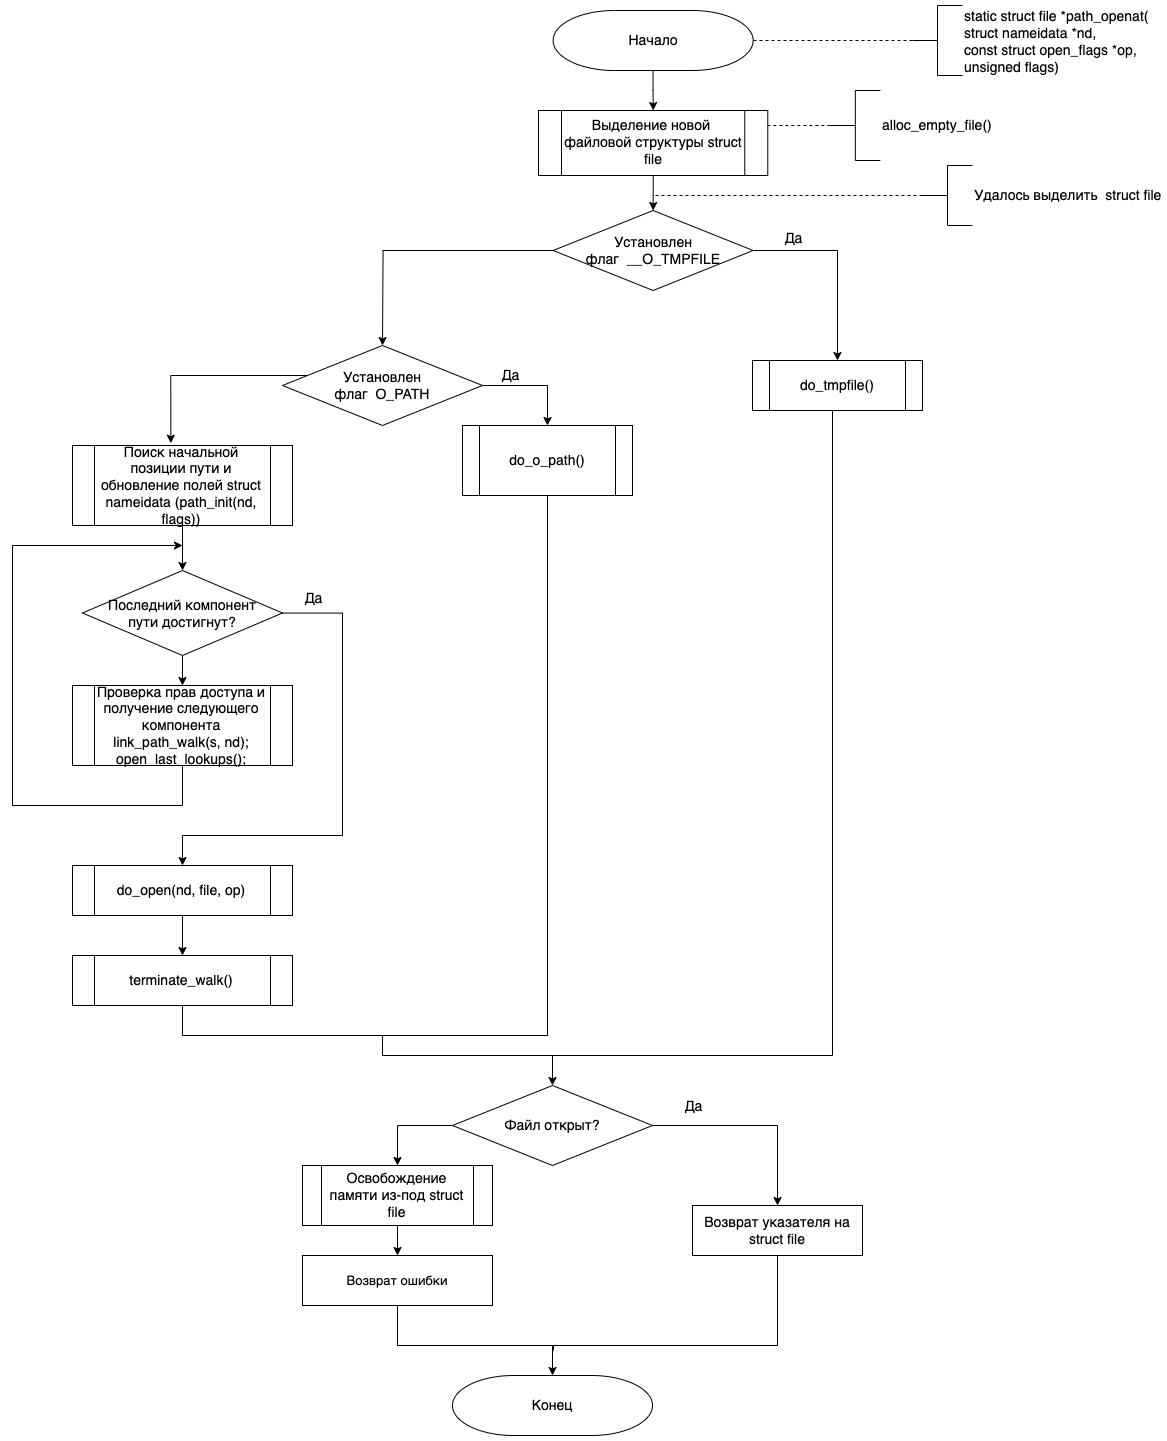
\includegraphics[width=\textwidth]{images/path_openat}
	\end{center}
	\caption{Схема алгоритма работы функции path\_openat()}
	\label{img:openat}
\end{figure}

\begin{figure}[h!]
	\begin{center}
		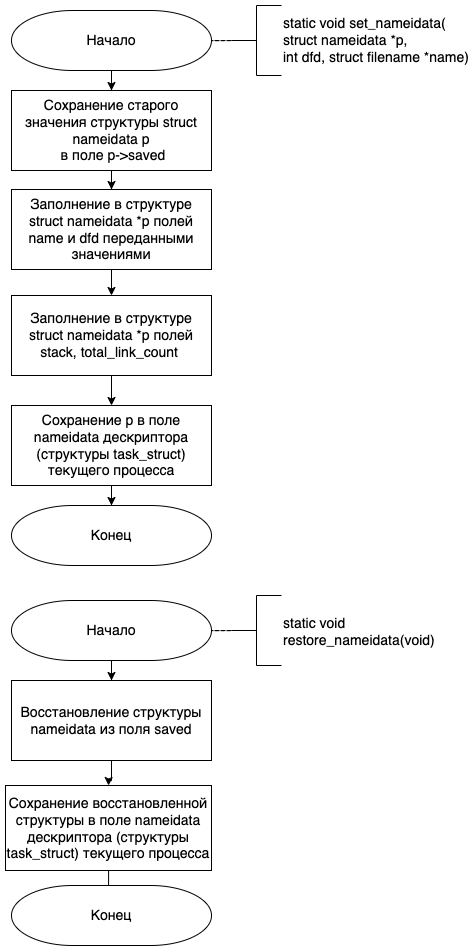
\includegraphics[width=120mm]{images/nameidata}
	\end{center}
	\caption{Схема алгоритма работы функций, работающих с nameidata}
	\label{img:name}
\end{figure}


\begin{figure}[h!]
	\begin{center}
		\includegraphics[width=\textwidth]{images/open\_last\_lookups}
	\end{center}
	\caption{Схема алгоритма работы функции open\_last\_lookups}
	\label{img:look}
\end{figure}

\begin{figure}[h!]
	\begin{center}
		\includegraphics[width=130mm]{images/lookup\_open}
	\end{center}
	\caption{Схема алгоритма работы функции lookup\_open}
	\label{img:lookup}
\end{figure}


